%% Ternary complex dimer Cartesian squares
%% FigS5TCDimerCartesianSquares.tex
%% Unused packages and definitions removed; TikZ/PGFPlots source formatted.

\documentclass[tikz,margin=2mm]{standalone}

\usepackage{amsfonts}

\def \half {\frac{1}{2}}

\begin{document}

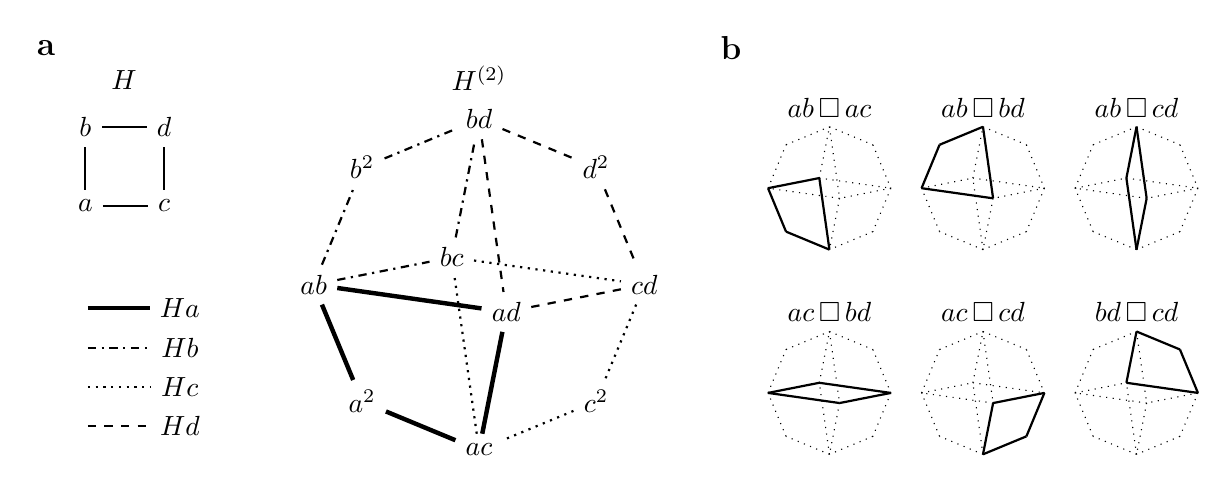
\begin{tikzpicture}[scale=1,style=thick,shorten >=0pt,shorten <=0pt]

    \begin{scope}[xshift=-7.5cm,yshift=-1.5cm,node distance=1cm]
        \node (LRA) {$b$};
        \node[below of=LRA] (RA) {$a$};
        \draw[thick] (LRA) to  (RA);
        \node[right of=RA] (RAG) {$c$};
        \draw[thick] (RA) to  (RAG);
        \node[right of=LRA] (LRAG) {$d$};
        \draw[thick] (LRAG) to (LRA);
        \draw[thick] (RAG) to  (LRAG);
        \path (LRA) to node[above,yshift=10pt] {$H$} (LRAG);
    \end{scope}

    \begin{scope}[xshift=-6.3cm,yshift=-3.8cm,node distance=1.3cm]
        \draw (0,0) node[] (Ha) {$Ha$};
        \node[left of=Ha] (HaL) {};
        \draw[ultra thick] (HaL) -- (Ha);
        \draw (0,-0.5) node[] (Hb) {$Hb$};
        \node[left of=Hb] (HbL) {};
        \draw[dashdotted] (HbL) -- (Hb);
        \draw (0,-1.0) node[] (Hc) {$Hc$};
        \node[left of=Hc] (HcL) {};
        \draw[dotted] (HcL) -- (Hc);
        \draw (0,-1.5) node[] (Hd) {$Hd$};
        \node[left of=Hd] (HdL) {};
        \draw[dashed] (HdL) -- (Hd);

        %\node[below of = LRA] (RA) {$a$};
        %\draw [thick] (LRA) to  (RA);
        %\node[right of = RA] (RAG) {$c$};
        %\draw [thick] (RA) to  (RAG);
        %\node[right of = LRA] (LRAG) {$d$};
        %\draw [thick] (LRAG) to (LRA);
        %\draw [thick] (RAG) to  (LRAG);
        %\path (LRA) to node[above,yshift=10pt] {$H$} (LRAG);
    \end{scope}

    \begin{scope}[xshift=-2.5cm,yshift=-3.5cm,scale=0.7,shorten >=0pt,shorten <=0pt]
        \coordinate (title) at (90:3.75);
        %\draw (title) node {$H^{(2)}=(H\,\Box\, H)/S_2$};
        \draw (title) node {$H^{(2)}$};
        \draw (0:3) node[] (cd) {$cd$};
        \draw (45:3) node[] (d2) {$d^2$};
        \draw (90:3) node[] (bd) {$bd$};
        \draw (135:3) node[] (b2) {$b^2$};
        \draw (180:3) node[] (ab) {$ab$};
        \draw (225:3) node[] (a2) {$a^2$};
        \draw (270:3) node[] (ac) {$ac$};
        \draw (315:3) node[] (c2) {$c^2$};
        \draw (315:0.7) node[] (ad) {$ad$};
        \draw (135:0.7) node[] (bc) {$bc$};
        \draw[ultra thick] (a2) -- (ab);
        \draw[dashdotted] (ab) -- (b2);
        \draw[dashdotted] (b2) -- (bd);
        \draw[dashed] (bd) -- (d2);
        \draw[dashed] (d2) -- (cd);
        \draw[dotted] (cd) -- (c2);
        \draw[dotted] (c2) -- (ac);
        \draw[ultra thick] (ac) -- (a2);
        \draw[dashdotted] (bc) -- (bd);
        \draw[dashed] (bd) -- (ad);
        \draw[ultra thick] (ad) -- (ac);
        \draw[dotted] (ac) -- (bc);
        \draw[dashdotted] (ab) -- (bc);
        \draw[dotted] (bc)-- (cd);
        \draw[dashed] (cd) -- (ad);
        \draw[ultra thick] (ad)-- (ab);
    \end{scope}

    \begin{scope}[scale=0.65,xshift=-2cm,yshift=-7.5cm,thin]
        \begin{scope}[xshift=5cm,yshift=0cm,scale=0.4]
            \coordinate (cd) at (0:3);
            \coordinate (d2) at (45:3);
            \coordinate (bd) at  (90:3);
            \coordinate (b2) at  (135:3);
            \coordinate (ab) at  (180:3);
            \coordinate (a2) at  (225:3);
            \coordinate (ac) at  (270:3);
            \coordinate (c2) at  (315:3);
            \coordinate (ad) at  (315:0.7);
            \coordinate (bc) at  (135:0.7);

            \draw[dotted] (a2) -- (ab);
            \draw[dotted] (ab) -- (b2);
            \draw[dotted] (b2) -- (bd);
            \draw[dotted] (bd) -- (d2);
            \draw[dotted] (d2) -- (cd);
            \draw[dotted] (cd) -- (c2);
            \draw[dotted] (c2) -- (ac);
            \draw[dotted] (ac) -- (a2);
            \draw[dotted] (bc) -- (bd);
            \draw[dotted] (bd) -- (ad);
            \draw[dotted] (ad) -- (ac);
            \draw[dotted] (ac) -- (bc);
            \draw[thick] (ab) -- (bc);
            \draw[thick] (bc) -- (cd);
            \draw[thick] (cd) -- (ad);
            \draw[thick] (ad) -- (ab);
            \draw (bd) node[above] {$ac\,\Box\, bd$};
        \end{scope}

        \begin{scope}[xshift=8cm,yshift=0cm,scale=0.4]
            \coordinate (cd) at (0:3);
            \coordinate (d2) at (45:3);
            \coordinate (bd) at  (90:3);
            \coordinate (b2) at  (135:3);
            \coordinate (ab) at  (180:3);
            \coordinate (a2) at  (225:3);
            \coordinate (ac) at  (270:3);
            \coordinate (c2) at  (315:3);
            \coordinate (ad) at  (315:0.7);
            \coordinate (bc) at  (135:0.7);

            \draw[dotted] (a2) -- (ab);
            \draw[dotted] (ab) -- (b2);
            \draw[dotted] (b2) -- (bd);
            \draw[dotted] (bd) -- (d2);
            \draw[dotted] (d2) -- (cd);
            \draw[thick] (cd) -- (c2);
            \draw[thick] (c2) -- (ac);
            \draw[dotted] (ac) -- (a2);
            \draw[dotted] (bc) -- (bd);
            \draw[dotted] (bd) -- (ad);
            \draw[thick] (ad) -- (ac);
            \draw[dotted] (ac) -- (bc);
            \draw[dotted] (ab) -- (bc);
            \draw[dotted] (bc) -- (cd);
            \draw[thick] (cd) -- (ad);
            \draw[dotted] (ad) -- (ab);
            \draw (bd) node[above] {$ac\,\Box\, cd$};
        \end{scope}

        \begin{scope}[xshift=11cm,yshift=0cm,scale=0.4]
            \coordinate (cd) at (0:3);
            \coordinate (d2) at (45:3);
            \coordinate (bd) at  (90:3);
            \coordinate (b2) at  (135:3);
            \coordinate (ab) at  (180:3);
            \coordinate (a2) at  (225:3);
            \coordinate (ac) at  (270:3);
            \coordinate (c2) at  (315:3);
            \coordinate (ad) at  (315:0.7);
            \coordinate (bc) at  (135:0.7);

            \draw[dotted] (a2) -- (ab);
            \draw[dotted] (ab) -- (b2);
            \draw[dotted] (b2) -- (bd);
            \draw[thick] (bd) -- (d2);
            \draw[thick] (d2) -- (cd);
            \draw[dotted] (cd) -- (c2);
            \draw[dotted] (c2) -- (ac);
            \draw[dotted] (ac) -- (a2);
            \draw[thick] (bc) -- (bd);
            \draw[dotted] (bd) -- (ad);
            \draw[dotted] (ad) -- (ac);
            \draw[dotted] (ac) -- (bc);
            \draw[dotted] (ab) -- (bc);
            \draw[thick] (bc) -- (cd);
            \draw[dotted] (cd) -- (ad);
            \draw[dotted] (ad) -- (ab);
            \draw (bd) node[above] {$bd\,\Box\, cd$};
        \end{scope}

        \begin{scope}[xshift=5cm,yshift=4cm,scale=0.4]
            \coordinate (cd) at (0:3);
            \coordinate (d2) at (45:3);
            \coordinate (bd) at  (90:3);
            \coordinate (b2) at  (135:3);
            \coordinate (ab) at  (180:3);
            \coordinate (a2) at  (225:3);
            \coordinate (ac) at  (270:3);
            \coordinate (c2) at  (315:3);
            \coordinate (ad) at  (315:0.7);
            \coordinate (bc) at  (135:0.7);

            \draw[thick] (a2) -- (ab);
            \draw[dotted] (ab) -- (b2);
            \draw[dotted] (b2) -- (bd);
            \draw[dotted] (bd) -- (d2);
            \draw[dotted] (d2) -- (cd);
            \draw[dotted] (cd) -- (c2);
            \draw[dotted] (c2) -- (ac);
            \draw[thick] (ac) -- (a2);
            \draw[dotted] (bc) -- (bd);
            \draw[dotted] (bd) -- (ad);
            \draw[dotted] (ad) -- (ac);
            \draw[thick] (ac) -- (bc);
            \draw[thick] (ab) -- (bc);
            \draw[dotted] (bc) -- (cd);
            \draw[dotted] (cd) -- (ad);
            \draw[dotted] (ad) -- (ab);
            \draw (bd) node[above] {$ab\,\Box\, ac$};
        \end{scope}

        \begin{scope}[xshift=8cm,yshift=4cm,scale=0.4]
            \coordinate (cd) at (0:3);
            \coordinate (d2) at (45:3);
            \coordinate (bd) at  (90:3);
            \coordinate (b2) at  (135:3);
            \coordinate (ab) at  (180:3);
            \coordinate (a2) at  (225:3);
            \coordinate (ac) at  (270:3);
            \coordinate (c2) at  (315:3);
            \coordinate (ad) at  (315:0.7);
            \coordinate (bc) at  (135:0.7);

            \draw[dotted] (a2) -- (ab);
            \draw[thick] (ab) -- (b2);
            \draw[thick] (b2) -- (bd);
            \draw[dotted] (bd) -- (d2);
            \draw[dotted] (d2) -- (cd);
            \draw[dotted] (cd) -- (c2);
            \draw[dotted] (c2) -- (ac);
            \draw[dotted] (ac) -- (a2);
            \draw[dotted] (bc) -- (bd);
            \draw[thick] (bd) -- (ad);
            \draw[dotted] (ad) -- (ac);
            \draw[dotted] (ac) -- (bc);
            \draw[dotted] (ab) -- (bc);
            \draw[dotted] (bc) -- (cd);
            \draw[dotted] (cd) -- (ad);
            \draw[thick] (ad) -- (ab);
            \draw (bd) node[above] {$ab\,\Box\, bd$};
        \end{scope}

        \begin{scope}[xshift=11cm,yshift=4cm,scale=0.4]
            \coordinate (cd) at (0:3);
            \coordinate (d2) at (45:3);
            \coordinate (bd) at  (90:3);
            \coordinate (b2) at  (135:3);
            \coordinate (ab) at  (180:3);
            \coordinate (a2) at  (225:3);
            \coordinate (ac) at  (270:3);
            \coordinate (c2) at  (315:3);
            \coordinate (ad) at  (315:0.7);
            \coordinate (bc) at  (135:0.7);

            \draw[dotted] (a2) -- (ab);
            \draw[dotted] (ab) -- (b2);
            \draw[dotted] (b2) -- (bd);
            \draw[dotted] (bd) -- (d2);
            \draw[dotted] (d2) -- (cd);
            \draw[dotted] (cd) -- (c2);
            \draw[dotted] (c2) -- (ac);
            \draw[dotted] (ac) -- (a2);
            \draw[thick] (bc) -- (bd);
            \draw[thick] (bd) -- (ad);
            \draw[thick] (ad) -- (ac);
            \draw[thick] (ac) -- (bc);
            \draw[dotted] (ab) -- (bc);
            \draw[dotted] (bc) -- (cd);
            \draw[dotted] (cd) -- (ad);
            \draw[dotted] (ad) -- (ab);
            \draw (bd) node[above] {$ab\,\Box\, cd$};
        \end{scope}
    \end{scope}

    \def\height{-0.5}
    \def\left{-8}
    \draw (\left,\height) node[font=\large] {{\bf a}};
    \draw (\left+8.7,\height) node[font=\large] {{\bf b}};
\end{tikzpicture}

\end{document}

